%% ------------------------------------------------------------------------- %%
\chapter{Processo de engenharia de software}
\label{cap:processoengenharia}

Processo de Engenharia de Software é uma sequência coerente de práticas que objetiva o desenvolvimento ou evolução de sistemas de software. Estas práticas englobam as atividades de especificação, projeto, desenvolvimento, testes e caracterizam-se pela interação de ferramentas, pessoas e métodos \cite{engsoftiki:17}.

O processo de engenharia de software corresponde à definição, desenvolvimento, medição, gerenciamento, mudança e melhoria dos próprios processos de software \cite{SWEBOK2004}.

A definição de processo pode ser um procedimento, uma política, ou uma norma. Processos de ciclo de vida de software são definidos por uma série de razões, incluindo o incremento da qualidade do produto, melhorias da compreensão humana e comunicação, apoio ao processo de melhoria, apoio aos processos de gestão, orientação aos processos automatizados, e providenciando a execução de suporte automatizado \cite{SWEBOK2004}. 

Os tipos de definições exigidas no processo dependerão, pelo menos parcialmente, do motivo da definição. Também é importante notar que o contexto do projeto e da organização irão determinar a definição do tipo de processo que é mais útil. Variáveis importantes a considerar incluem a natureza do trabalho (por exemplo, a manutenção ou desenvolvimento), o domínio da aplicação, o modelo do ciclo de vida, e da maturidade da organização. \cite{SWEBOK2004}.

O principal objetivo é apresentar um modelo de processo de software apropriado para o estudo de caso \textit{"Restaurante Da Gino"} a partir da adaptação da ISO/IEC 12207:1995.

\section{Ciclo de vida e modelo de processo}
\label{sec:modelodeprocesso}

Um modelo de processo de software, ou simplesmente modelo de processo, pode ser visto como uma representação abstrata de um processo de software, apresentando a descrição do processo segundo uma perspectiva particular. Além disso, oferece uma forma mais abrangente e fácil de representar o gerenciamento de processo de software e consequentemente o progresso do projeto \cite{engsoftiki:17}.

O modelo de ciclo de vida que corresponde ao modelo de processo, é uma estrutura contendo processos, atividades e tarefas envolvidas no desenvolvimento, operação e manutenção de um produto de software, abrangendo a vida do sistema desde a definição de seus requisitos até o término de seu uso \cite{iso12207:95}.

Para definir o modelo de processo a ser adotado, foi necessário definir os critérios de seleção e analisá-las sob a perspectiva do adquirente e fornecedor, no caso, restaurante \textit{Da Gino} e a empresa de desenvolvimento de software, respectivamente.


\subsection{Quadro de referência do ciclo de vida do software}

Os principais fatores que foram analisados para a adaptação da ISO/IEC 12207:1995 que servirá de quadro de referência do ciclo de vida de software foram:

\begin{description}
  \item [Organizacionais] As políticas das organizações em questão, que neste caso seriam a empresa contratada para o desenvolvimento do projeto e o adquirente (Gino);
  \item [Documentação que deve ser gerada para o produto] Analisamos algumas necessidades e também informações disponibilizadas pelo adquirente;
  \item [Características do projeto] Analisamos algumas características do projeto a ser desenvolvido:
  \begin{itemize}
    \item Criticidade
    \item Tamanho
    \item Visibilidade
    \item Prazos de tempo e custo
    \item Requisitos do sistema
  \end{itemize}

\end{description}

\subsubsection{Definição do modelo de processo}

O modelo de processo que definimos para o desenvolvimento do software do restaurante \textit{Da Gino} foi um modelo de processo baseado nas características dos modelos ágeis, cujas principais características são um processo iterativo que organiza-se através do desenvolvimento baseado em entregas frequentes em curtos períodos de tempo, e também é guiado por boas práticas para inúmeros processos como documentação, desenvolvimento, comunicação e gerenciamento em geral. Analisando a definição frente a um modelo de ciclo de vida foi escolhido o modelo de processo baseado em métodos ágeis Scrum.

\subsubsection{Justificativa para a adoção do Modelo de Processo}

Com relação ao fator organizacional verificou-se que o Restaurante \textit{Da Gino} encontra-se em pré-construção tanto de sua parte física quanto dos processos lógicos que regeriam a organização e como hipótese assumida definimos que os processos de regras organizacionais seriam processos de grande maleabilidade e fácil adaptação. 

A empresa responsável pelo desenvolvimento do sistema é uma fábrica de software e possui como principal regra organizacional o fator produtividade, portanto o desenvolvimento de sistemas é baseado principalmente em entregas frequentes em pequenos intervalos de tempo. 

A partir disto, conclui-se que as duas empresas apresentam uma grande flexibilidade e desejam ter um sistema funcionando em um curto espaço de tempo. 

Já com relação a documentação, assumiremos que os documentos exigidos pelo adquirente são documentos de baixa complexidade e que somente refletem as formas de utilização do sistema, como por exemplo, um manual final de utilização do sistema. Do lado da empresa desenvolvedora em função dos objetivos  finais fica claro que neste caso quanto mais específica for a documentação permitindo que o desenvolvimento seja realizado é o suficiente, ou seja, a documentação precisa auxiliar principalmente o desenvolvimento e não as outras equipes como qualidade, de teste e gerenciamento.

Analisando as principais características do produto a ser desenvolvido, temos:

\begin{description}
  \item [Criticidade e Visibilidade] o software a ser desenvolvido não é um sistema crítico e não será um sistema que irá alavancar o nome de uma empresa, portanto não possui grande visibilidade como produto para o restaurante \textit{Da Gino}. Logo, não há a necessidade de empresas terceiras que avaliem a qualidade, inspecionem os códigos e as funcionalidades ou que valide com extrema cautela através de processos específicos, pois este papel poderá ser realizado pelo própria equipe desenvolvedora.
  \item [Prazos de tempo e custo] Assumiremos que o projeto tem um custo reduzido para ser desenvolvido por volta R\$ 350.000,00 para ser utilizado na compra de equipamentos eletrônicos, computadores, monitores e custear todo o projeto, além disso necessita que seja desenvolvido e terminado com restrições de tempo, cerca de 6 meses. A partir desta premissa, é necessário escolher um modelo de processo que permita desenvolver uma aplicação com uma equipe reduzida de no máximo cinco pessoas, com média a alta experiência e que seja auto-sustentável, organizável, e possuam facilidade na troca de informações.

  \item [Requisitos do sistema] os requisitos do sistema não são complexos, no entanto serão todos passados pelo dono do restaurante que no caso não possui conhecimento nenhum na área de sistemas, portanto concluímos que os requisitos são altamente mutáveis e podem estar incompletos o que irá refletir na equipe de desenvolvimento que por sua vez precisa ser capaz de gerenciar com sucesso às frequentes mudanças dos requisitos.
\end{description}

A partir das análises das principais características do produto, dos aspectos organizacionais e da documentação, concluímos o modelo de processo baseado em metodologias ágeis é o mais adequado. O modelo de processo ágil adotado será o \textit{Scrum}. O princípio chave do \textit{Scrum} é o reconhecimento que os clientes irão mudar de idéia sobre o que eles precisam e querem e que estas mudanças são imprevisíveis. A partir disso, o \textit{Scrum} foca em como maximizar as habilidades do time para fazer entregas mais rápido, para responder a alterações nos requisitos e para adaptar-se ao avanço das tecnologias e mudanças do mercado \cite{scrumwiki:17}.

%% ------------------------------------------------------------------------- %%

\subsection{Atividades do quadro de referência}
O modelo de processo ágil \textit{Scrum} é um arcabouço para gerenciar desenvolvimento de produtos. Logo, o Scrum não define boa parte das atividades e processos do quadro de referência da ISO/IEC 12207:1995. 

Porém, o Scrum mostrou-se o modelo de processo mais adequado dado as características do produto e aspectos organizacionais no nosso caso. 

Então, para definir as atividades do quadro de referência, iremos adotar os princípios e valores do Scrum e metodologias ágeis. Princípios e valores definidos no manifesto ágil\cite{beck2001agile}, no Scrum Guide\cite{Schw01a} e no livro Extreme Programming Explained: Embrace Change (2nd Edition)\cite{BecAnd04extreme}.

A nossa proposta de programa de Engenharia de Software irá abranger as seguintes áreas de conhecimento e contemplará as seguintes atividades a partir do quadro de referência adaptado da ISO/IEC 12207:1995 \cite{iso12207:95}:

\begin{description}
  \item [Processo de aquisição] Principais necessidades do adquirente são padronizar catálogo de receitas, controle de estoque e controle de disponibilidade de mesas.
  \begin{itemize}
    \item Iniciação - O adquirente irá manter um acordo com o fornecedor para a definição e análise dos requisitos do software devido ao pouco conhecimento sobre o assunto.
  \end{itemize}
  \item [Processo de fornecimento] O fornecedor será responsável por analisar todos os requisitos do sistema de acordo com as necessidades levantadas pelo adquirente (Gino), através de um acordo de contrato.
  \begin{itemize}
    \item Iniciação
    \item Preparação de resposta
    \item Contrato
    \item Planejamento
    \item Execução e controle
    \item Revisão e avaliação
    \item Entrega e conclusão
  \end{itemize}
  \item [Processo de desenvolvimento] A empresa adota práticas e métodos ágeis com o objetivo de maximizar o processo de codificação e testes.
  \begin{itemize}
    \item Implementação do processo
    \item Análise dos Requisitos do Sistema e Análise dos requisitos de software
    \item Projeto de arquitetura do sistema e projeto de arquitetura do software
    \item Projeto detalhado do software
    \item Codificação e Teste do software / Integração do software e Integração do sistema
    \item Teste de quali cação do software e Teste de quali cação do sistema
    \item Instalação do software e Apoio à aceitação do software
  \end{itemize}
  \item [Processo de operação e Manutenção] O intuito é que o desenvolvimento seja guiado por testes, sendo que esta prática garante que os erros sejam descobertos rapidamente, com isso, manutenção corretiva é colocada em prática para prevenir ou reduzir a necessidade deste tipo de manutenção depois que o produto foi entregue ao cliente. 
\end{description}

\subsection{Modelo de processo de software}

\subsubsection{\large{Processo de aquisição}}

Segundo a NBR ISO/IEC 12207:1998 \cite{iso12207:95}, o processo de aquisição é composto pelas seguintes atividades:

\begin{enumerate}
  \item Iniciação
  \item Preparação de pedido de proposta
  \item Preparação e atualização do contrato
  \item Monitoração do fornecedor
  \item Aceitação e conclusão
\end{enumerate}

Segundo o item 5.1.1.1 da ISO \cite{iso12207:95}, o adquirente (Gino) inicia o processo com a
descrição de um conceito ou necessidade a adquirir. Principais necessidades do adquirente são:

\begin{itemize}
  \item Padronizar catálogo de receitas
  \item Controle de estoque
  \item Controle de disponibilidade de mesas
\end{itemize}

Segundo o item 5.1.1.4, o adquirente (Gino) pode executar a definição e a análise dos requisitos do software por conta própria ou pode manter acordo com um fornecedor para executar essa tarefa. O adquirente optou por manter um acordo com a empresa de software para que seja feita a definição e análise dos requisitos. Documento de visão será criado para detalhar melhor os requisitos e a estrutura organizacional.

\begin{table}[htb]
      \begin{center}
        \begin{tabular}{| l | l | l | l |}
        \hline
        \textbf{Atividade} & \textbf{Cobertura} \\ \hline
        Iniciação & Parcial \\ \hline
        Preparação de pedido de proposta & Não contempla \\ \hline
        Preparação e atualização do contrato & Não contempla \\ \hline
        Monitoração do fornecedor & Não contempla \\ \hline
        Aceitação e conclusão & Não contempla \\ \hline
        \end{tabular}
      \end{center}
    \caption{Cobertura das atividades do processo de aquisição}
    \end{table}



%% ------------------------------------------------------------------------- %%
\subsubsection{\large{Processo de fornecimento}}
\label{sec:fornecimento}

O fornecedor será responsável por analisar todos os requisitos do sistema de acordo com as necessidades levantadas pelo adquirente (Gino), através de um acordo de contrato. A proposta de tipo de contrato terá escopo variável. Quanto à responsabilidade das organizações, o fornecedor deverá atender as necessidades estabelecidas pelo adquirente para o aceite do software desenvolvido e é de responsabilidade do adquirente prover todas as informações e dados ao fornecedor para a definição do produto final.
O fornecedor será responsável por realizar toda a preparação necessária para elaboração do pedido de proposta do cliente, neste caso, o Gino.

Para a elaboração do pedido de proposta, o fornecedor tem a responsabilidade pelos seguintes itens \cite{iso12207:95}:
\begin{itemize}
  \item Requisitos do sistema
  \item Declaração do escopo
  \item Lista de produtos de software
  \item Termos e condições
  \item Restrições técnicas
\end{itemize}

Após prover os itens acima, eles só serão validados mediante aprovação do cliente.

O contrato será confeccionado mediante direitos de uso, de propriedade, de autoria, de garantia e de licença \cite{iso12207:95}. O adquirente terá prioridade no suporte da aplicação por período pré-estabelecido entre as partes. Também fica pré-definido que qualquer alteração ou aditivo que ocorra no contrato, o fornecedor e o adquirente devem estar em comum acordo. Um documento aprovado por ambas as partes deve ser elaborado suportando estas modificações: análise de impacto quanto a prazos, cronograma e custos \cite{iso12207:95}.

A aceitação será realizada de acordo com o descrito em cada item de requisito levantado, durante as entregas parciais. Uma vez que o fornecedor faz uso de um modelo de desenvolvimento que prevê entregas parciais, o adquirente poderá fazer a validação, verificação e aceitação destas entregas evoluindo até a aceitação final do projeto. A monitoração será realizada de acordo com os status das entregas parciais providas pelo fornecedor. 

Segue a descrição das tarefas e atividades do fornecedor para o processo de fornecimento:


\subparagraph{Iniciação}

Fornecedor conduzirá uma revisão das necessidades levantadas pelo adquirente para decidir ou propor mudanças para a aceitação do contrato (5.2.1.1 e 5.2.1.2) \cite{iso12207:95}.

\subparagraph{Preparação de resposta}

O fornecedor será responsável por definir todos os requisitos em resposta ao pedido do \textit{Gino}.

\subparagraph{Contrato}

Contrato terá escopo variável para atender as necessidades do adquirente de acordo com suas prioridades e trabalhar de acordo com o modelo de desenvolvimento da empresa, Scrum.

\subparagraph{Planejamento}

\begin{itemize}
  \item Recursos internos para o desenvolvimento do software utilizando o modelo iterativo Scrum (5.2.4.4)
  \item Requisitos e prioridades serão descritos pelo documento de Visão (5.2.4.1)
  \item Estrutura organizacional e cada ciclo será definido pelo Scrum (5.2.4.2 e 5.2.4.5 a.)
  \item Uso do Kanban e diagrama de Burndown para realizar acompanhamento do progresso (5.2.4.5 n.)
  \item Estes diagramas de \textit{Burndown} poderão ser disponibilizados periodicamente ao adquirente para acompanhamento do progresso
  \item Será provido treinamento ao adquirente para a utilização do produto do software (5.2.4.5 o.)
\end{itemize}

\subparagraph{Execução e controle}

Monitoramento de progresso feito por Kanban e Burndown (5.2.5.3).

\subparagraph{Revisão e avaliação}

Fornecedor fará uso de um modelo de entregas parciais. O adquirente irá revisar de acordo com a descrição em cada item de requisito levantando durante as entregas parciais. 

\subparagraph{Entrega e conclusão}

O modelo de processo adotado baseia-se em entregas frequentes de versões do produto que sejam completos e utilizáveis. Quer dizer, o cliente ao final de cada entrega terá uma versão do produto que já pode ser utilizada. O adquirente fará a validação e aceitação das entregas parciais evoluindo até a aceitação do produto final.


    \begin{table}[htb]
      \begin{center}
        \begin{tabular}{| l | l | l | l |}
        \hline
        \textbf{Atividade} & \textbf{Cobertura} \\ \hline
        Iniciação & Parcial \\ \hline
        Preparação de resposta & Total \\ \hline
        Contrato & Total \\ \hline
        Planejamento & Total \\ \hline
        Execução e controle & Total \\ \hline
        Revisão e avaliação & Parcial \\ \hline
        Entrega e conclusão & Parcial \\ \hline
        \end{tabular}
      \end{center}
    \caption{Cobertura das atividades do processo de fornecimento}
    \end{table}



%% ------------------------------------------------------------------------- %%
\subsubsection{\large{Processo de desenvolvimento}}
\label{sec:desenvolvimento}

Segue uma descrição das atividades e tarefas do processo de desenvolvimento:

\subparagraph{Implementação do processo}

O Scrum é um modelo de processo ágil iterativo e incremental para gerenciamento de desenvolvimento de produto \cite{scrumwiki:17}. O Scrum contém práticas bem definidas que devem ser seguidas pela equipe e organização. As práticas são fáceis de aprender, porém são difíceis de dominar \cite{Schw01a}. 

A equipe do Scrum é formado pelo Scrum Master, Product Owner e o time de desenvolvimento. O tamanho da equipe de desenvolvimento não deve ser menor que 3 pessoas, pois caso a equipe seja pequena pode ter problemas durante a Sprint e não ser capaz de entregar os incrementos do produto. A equipe não deve exceder 9 pessoas, pois uma equipe grande é difícil de coordenar \cite{Schw01a}. O tamanho ideal da equipe de desenvolvimento é de 3 a 9 pessoas.

Todo o processo será baseado em valores, princípios que norteiam tanto o processo quanto as políticas de gerência, manutenção e qualidade.

Para a correta implementação do processo, os desenvolvedores e gerentes deverão ler o livro do Scrum.

\begin{figure}[!h]
  \centering
  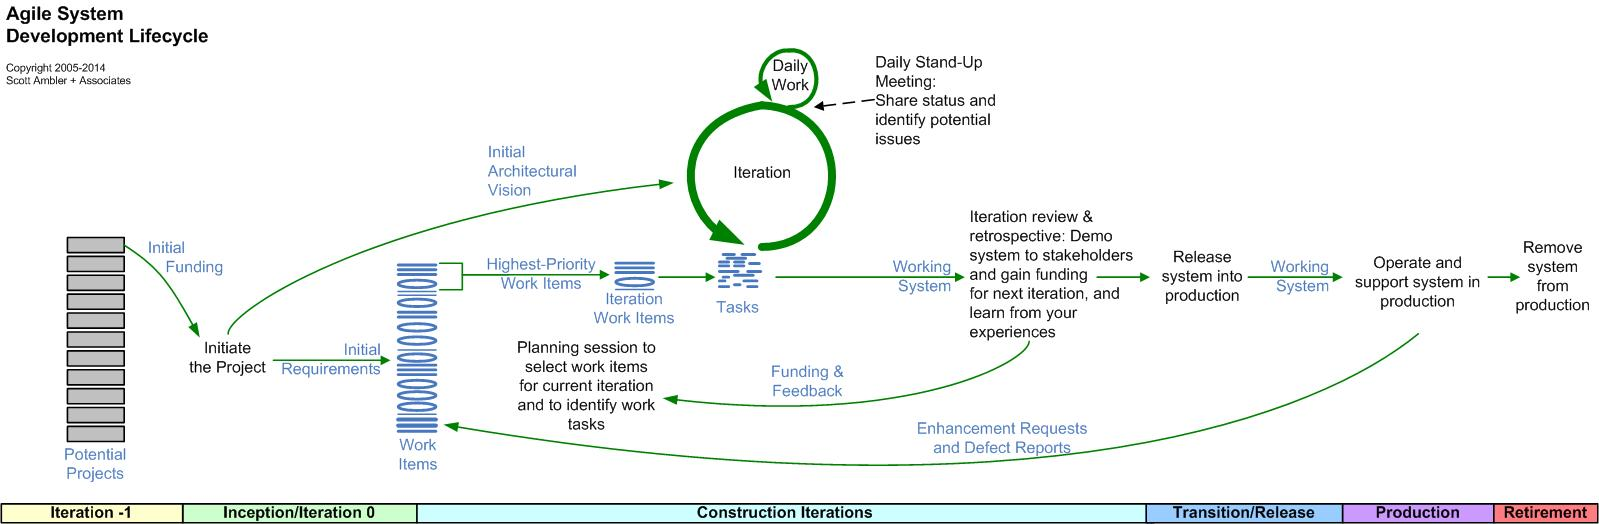
\includegraphics[width=1\textwidth]{softwareengineer/images/agileLifecycleDetailed} 
  \caption{Seleção do ciclo de vida ágil baseado no Scrum \cite{ambysoft:09}}
  \label{fig:scrumlifecycle} 
\end{figure}

\subparagraph{Análise dos Requisitos do Sistema e Análise dos requisitos de software}

\begin{itemize}
  \item Os requisitos serão definidos pelo fornecedor de acordo com as necessidades levantadas pelo adquirente

  \item Todos os requisitos serão definidos e listados no Product Backlog

  \item Eles serão listados e priorizados pelo PO (Product Owner) e Scrum Master antes do Sprint Planning
\end{itemize}

\subparagraph{Projeto de arquitetura do sistema e Projeto de arquitetura do software}

Estas duas atividades são compostas pelos processos de análise de requisitos pelo modelo de ciclo de vida, pois durante as atividades de análise na qual o Product Owner e o cliente geram todas as estórias que seriam os módulos ou casos de uso ou funcionalidades do sistema, parte da equipe técnica se concentrará em definir os requisitos e outra parte em definir como o sistema deveria ser "\textit{montado}". Especialistas em arquitetura de sistemas desenvolveriam modelos arquiteturais que correspondessem as necessidades do projeto ao mesmo tempo em que analistas de negócios e projetistas de sistemas gerariam um projeto modularizado e componentizado montando assim uma arquitetura de como o software deve ser implementado.

\subparagraph{Projeto detalhado do software}

O modelo de ciclo de vida não prioriza o detalhamento em documentação do sistema e sim um modelo de implementação de funcionalidades que tenham sido previamente definidas e que serão complementadas pelas informações constantes do cliente que sempre estará em contato com a equipe.

\subparagraph{Codificação e Teste do software / Integração do software e Integração do sistema}


Isto é um ponto fraco do modelo de ciclo de vida. No Scrum não há definição de papéis na equipe de desenvolvimento, todos são desenvolvedores. Além disso, não há uma definição sobre as atividades de codificação, teste e integração. Neste caso, assumiremos que a empresa de software tem alguns procedimentos e práticas ágeis que a equipe de desenvolvimento deverá seguir. Os procedimentos a serem seguidos pela equipe de desenvolvimento visa otimizar ao máximo o processo de codificação e testes buscando um trabalho que seja auto-organizável e buscando também a formação de uma equipe que se auto-gerencia e se corrija.

O processos de gerenciamento ágil que evidencia os objetivos de foco no desenvolvimento e qualidade
dos testes afim de não gerar retrabalho e falhas futuras do software como:
\begin{itemize}
  \item Programação pareada para funcionalidades complexas e TDD (Test driven development).
  \item Todos os testes devem ser automatizados e executados várias vezes ao dia, com integração contínua;
  \item Comunicação é um fator de extrema importância tratado pelo manifesto ágil\cite{beck2001agile} com muito cuidado. Priorizam a comunicação falada e consequentemente documentada, pois consideram que esta é uma das melhores formas de passagem de conhecimento.
\end{itemize}

O processo de testes também será diferenciado, pois serão realizados dois tipos de testes, que são os unitários e ou automatizados e os testes de integração. Com isso, os erros tornam-se mais facilmente detectáveis e as soluções pra estes se tornam mais rápidas e precisas.

Frente a estas atividades, a integração do software e do sistema torna-se cada vez mais simples, já que todas estas atividades apóiam estas ultimas atividades citadas.






\subparagraph{Teste de qualificação do software e Teste de qualificação do sistema }

O modelo de ciclo de vida não define a atividade de teste e o fator de qualidade de testes do software e do sistema. No entanto, iremos assumir que a empresa adota práticas ágeis que objetivam ter qualidade em seus resultados e por isso sempre mantém o cliente como participante do processo.

\subparagraph{Instalação do software e Apoio à aceitação do software}

O modelo de ciclo de vida não define estas atividades. Neste caso, as práticas adotadas pela empresa será as práticas ágeis. A atividade de aceitação será completamente trabalhada no projeto, pois o principal interessado no projeto mantém-se presente durante todo o processo de entrega de incrementos do sistema, tirando dúvidas dos desenvolvedores realizando reuniões de acompanhamento de entregas como o Sprint Review. Para o processo de instalação assumiremos que os integrantes da equipe de maior conhecimento no sistema junto aos projetistas do sistema e do software são responsáveis junto a seus gerentes pela instalação do sistema, assim conclui-se que existe uma equipe mobilizada para a instalação e a realização da atividade com sucesso.

\begin{table}[htb]
      \begin{center}
        \begin{tabular}{| p{6cm} | l |}
        \hline
        \textbf{Atividade} & \textbf{Cobertura} \\ \hline
        Implementação do processo & Parcial \\ \hline
        Análise dos Requisitos do Sistema e Análise dos requisitos de software & Parcial \\ \hline
        Projeto de arquitetura do sistema e Projeto de arquitetura do software & Não contempla \\ \hline
        Projeto detalhado do software & Não contempla \\ \hline
        Codificação e Teste do software / Integração do software e Integração do sistema & Parcial \\ \hline
        Teste de qualificação do software e Teste de qualificação do sistema & Parcial \\ \hline
        Instalação do software e Apoio à aceitação do software & Parcial \\ \hline
        \end{tabular}
      \end{center}
    \caption{Cobertura das atividades do processo de desenvolvimento}
    \end{table}


\subsubsection{\large{Processo de Operação e Manutenção}}
\label{sec:operacao}

O processo de operação e manutenção ocorrem simultaneamente. O processo de operação consiste em auxilar os usuários no uso do produto recentemente criado \cite{iso12207:95}. A manutenção de software é a atividade durante a qual ocorrem modicações em um ou mais artefatos de software resultante do desenvolvimento de um software (ou de manutenções anteriores), buscando mantê-lo disponível, corrigir suas falhas, melhorar seu desempenho e adequá-lo aos requisitos novos ou modificados, conforme as necessidades de seus usuários\cite{IEEE1990}.

O intuito é que o desenvolvimento seja guiado por testes, sendo que esta prática garante que os erros sejam descobertos rapidamente, com isso, manutenção corretiva é colocada em prática para prevenir ou reduzir a necessidade deste tipo de manutenção depois que o produto foi entregue ao cliente.
Outra prática ágil é o refactoring que garante que uma futura manutenção software possa ser continuada facilmente, auxiliando a categoria de manutenção preventiva e perfectiva.
Outras práticas também auxiliam, como no caso de padrões de desenvolvimento e design simples.

Caso haja uma descontinuação do software, todos os artefatos gerados durante o ciclo de vida do processo de software serão disponibilizados ao cliente, bem como manuais ou qualquer outro documento que o adquirente tenha requisitado em comum acordo.

\begin{table}[htb]
      \begin{center}
        \begin{tabular}{| p{6cm} | l |}
        \hline
        \textbf{Atividade} & \textbf{Cobertura} \\ \hline
        Implementação do processo & Parcial \\ \hline
        Teste operacional & Não contempla \\ \hline
        Operação do sistema & Não contempla \\ \hline
        Suporte ao usuário & Parcial \\ \hline
        \end{tabular}
      \end{center}
    \caption{Cobertura das atividades do processo de operação}
    \end{table}

    \begin{table}[htb]
      \begin{center}
        \begin{tabular}{| p{6cm} | l |}
        \hline
        \textbf{Atividade} & \textbf{Cobertura} \\ \hline
        Implementação do processo & Parcial \\ \hline
        Análise do problema e da modificação & Parcial \\ \hline
        Implementação da modificação & Total\\ \hline
        Revisão/aceitação da manutenção & Parcial \\ \hline
        Migração & Não contempla \\ \hline
        Descontinuação do software & Parcial \\ \hline
        \end{tabular}
      \end{center}
    \caption{Cobertura das atividades do processo de manutenção}
    \end{table}

\section{Requisitos de Software}
\label{sec:requisitos}

\large{Seção de requisitos - Marcelo}

\subsection{Atividades e Papéis}

Em uma tabela, mapear as atividades definidas em 2.1.2
para requisitos de software nas atividades de requisitos de
software do processo selecionado em 2.1.3.


Definir as atividades e os papéis dos responsáveis
envolvidos do modelo de processo selecionado.

\subsection{Artefatos}

Definir os artefatos produzidos pelas atividades do processo
de software e dar um exemplo de cada artefato.

Definir e justificar a(s) técnica(s) de elicitação dos
requisitos de software que devem ser utilizadas.

\section{Qualidade de software}
\label{sec:qualisoftware}


\large{Seção de qualidade de software - Alex}

\subsection{Plano de garantia de qualidade de software}

Definir um plano de garantia de qualidade de software para
o modelo de processo definido em 2.1.3 que esteja em
conformidade com o padrão IEEE Std 730-2002 (ou IEEE
Std 730-2014).

Definir as tarefas de revisão deverão utilizar o IEEE Std
1028-2008:IEEE Standard for Software Reviews and Audits.

\subsection{Tarefas e papéis}

Detalhar as tarefas do plano de garantia de qualidade de
software definido no item anterior. Detalhar também os
papéis dos responsáveis envolvidos.

Definir os artefatos produzidos pelas tarefas e dar um
exemplo de artefato.



\section{Gerência da engenharia de software}
\label{sec:gerenciaengenharia}

\large{Seção gerência de engenharia de software - alex}

Assumir o modelo de processo de software e o plano de garantia
de qualidade de software definidos em 2.1.3 e 2.3.1.

\subsection{Estimativa do projeto}

Aplicar uma técnica de estimativa para o projeto do
exemplo da disciplina, explicando os detalhes desta
aplicação

Justificar a escolha, determinar os objetivos da estimativa e
discutir os resultados da estimativa.

\subsection{Planejamento do projeto}

Apresentar um esboço do planejamento do projeto
consistente com os resultados da estimativa acima e os
modelos e planos adotados em todo o trabalho.



\section{Gerência de configuração de software}
\label{sec:gerenciaconfig}

\large{Seção gerência de configuração de software - alex}

\subsection{Plano de gerência de configuração de software}

Definir um plano de gerência de configuração de software
para o modelo de processo definido em 2.1.3 e que esteja
em conformidade com o padrão IEEE Std 828-2005: IEEE
Standard for Software Configuration Management Plans ou
o IEEE Std 828-2012: IEEE Standard for Configuration
Management in Systems and Software Engineering.

\subsection{Tarefas e papéis}

Descrever as tarefas da gerência de configuração do plano
definido no item anterior. Descrever também os papéis dos
responsáveis envolvidos.

Definir os artefatos produzidos pelas tarefas e dar um
exemplo de artefato.



\section{Teste de software}
\label{sec:teste}

\large{Seção de teste de software - marcelo}

\subsection{Padrão para o Teste de Aceitação}

Considerando que o denominado “uso parcial” do padrão
IEEE Std 829-2008: IEEE Std for Software and System Test
Documentation atende ao padrão ISO/IEC 12207 (incluindo
a versão de 1995), apresentar:

– Uma configuração apropriada deste uso para o Teste de
Aceitação, levando-se em conta as características do exemplo
da disciplina, para os níveis de Planejamento, Projeto (design),
Caso de Teste e Procedimento do Teste.

\subsection{Definição do Teste de Aceitação}

Supor que as características do produto de software
estejam organizadas nas seguintes áreas de negócio do
restaurante: recepção ao cliente, serviço de refeição,
cozinha, pagamento e estoque.

Para cada área de negócio:
1. Definir todos os papéis e suas responsabilidades.
2. Definir os atributos dos papéis.
3. Definir uma característica do produto de software.
Para uma área de negócio selecionada:
4. Elaborar uma história de usuário para a característica definida,
utilizando o formato apresentado em aula.
5. Definir dois critérios de aceitação para a história.
6. Derivar um cenário abstrato correspondente para cada critério de
aceitação, usando os elementos básicos da linguagem Guerkin.
7. Derivar um cenário concreto, isto é, um caso de teste de aceitação, para
cada cenário abstrato definido usando a linguagem Guerkin.












